\documentclass[12pt,addpoints,answers]{exam}
\unframedsolutions
\renewcommand{\solutiontitle}{\noindent\textbf{Solution:}\par\noindent}
\SolutionEmphasis{\color{blue}}
%\noprintanswers
\usepackage[utf8]{inputenc}

\usepackage{booktabs}
\usepackage{tabularx}
\usepackage{multirow}
\usepackage{colortbl}
\usepackage{subcaption}
\usepackage{hyperref}
\usepackage{mathtools}
\usepackage{logicproof}
\usepackage[inline]{enumitem}
\usepackage{graphbox}
\usepackage{xfrac}
\usepackage{xspace}
\usepackage{bm}
\usepackage{tikz}
\usepackage{siunitx}

\usetikzlibrary{decorations}
\usetikzlibrary{decorations.pathreplacing}
\usetikzlibrary{positioning}
\usetikzlibrary{backgrounds}
\usetikzlibrary{matrix}
\usetikzlibrary{fit}
\usetikzlibrary{calc}
\usetikzlibrary{arrows}
\usetikzlibrary{shapes.geometric}
\usetikzlibrary{shapes.multipart}


% Used for code embed in problem 3
\usepackage{listings}
\usepackage{color}
\usepackage{amsmath}

% tables
\usepackage{multirow}
\usepackage{booktabs}

% Float fix
\usepackage{float}


\tikzset{
    position/.style args={#1:#2 from #3}{
        at=(#3.#1), anchor=#1+180, shift=(#1:#2)
    }
}

\setlength{\parindent}{0em}
\setlength{\parskip}{1em}

\DeclarePairedDelimiter{\abs}{\lvert}{\rvert}
\DeclarePairedDelimiter{\lvec}{\left\langle}{\right\rangle}
\DeclareMathOperator{\sign}{sign}
\DeclareMathOperator*{\argmax}{arg\,max}
\DeclareMathOperator*{\argmin}{arg\,min}

\newcommand{\astar}{A{\small{*}}\xspace}

\pagestyle{headandfoot}
\firstpageheader{\textbf{CS4461/EE4272}}{\textbf{Midterm Exam}}{\textbf{April 10st--April 13rd, 2020}}
\firstpageheadrule
\firstpagefooter{}{}{Page \thepage\ of \numpages}
\firstpagefootrule
\runningfooter{}{}{Page \thepage\ of \numpages}
\runningfootrule

\begin{document}
\vspace*{0.25in}
\begin{center}\Large{Exam Policies}\end{center}
\begin{itemize}
\item You will have a total of 96 hours to complete the exam: the exam releases at 12:00am on April 10st and the exam is due via submission to Canvas at 11:59pm on April 13rd.
\item You \textbf{may} use the textbook, the slides, your notes... any course material is fair game.
\item You \textbf{may not} cooperate with anyone else. This is a chance to prove \textbf{your} knowledge.
\item Use of calculators is fine for checking your answers. The same is true for programs that you may write yourself, or programs that you have written for this class. \textbf{You are still expected to show your work!}
\item This is designed as a typical exam, so it is designed for a 1 hour block of time to be taken in one sitting. I am giving you four days so that each of you can find your own time to work on the exam and to prepare your solutions for submission.
\item You are free to take as much time as you wish for the exam, but you should allocate at least 2 hours for completing your answers, and more if you need to type them up.
\item \textbf{Read questions in their entirety.}\\Questions may require multiple responses, including an explanation or a justification.
\end{itemize}
\vfill
\begin{center}\Large{Nondisclosure Agreement}\end{center}
\begin{itemize}
\item I attest that I am the person taking the exam.
\item I understand that I am on my honor to do my own work without any assistance from others or outside sources not allowed and agree that I will not disclose the contents of this exam.
\item If I am discovered to have compromised the exam in any way, I understand that I will receive a zero for the exam and will be referred to the Office of Student Affairs for violation of university policies regarding academic integrity.
\end{itemize}
\vspace*{0.25in}
\hrule
\vspace*{0.25in}
\textbf{By submitting this exam, I affirm that I have read, understand, and agree to the policies of this exam and the terms this agreement.}
\vspace*{0.25in}
\newpage

\begin{questions}

%%%
%%%
\question The following flows are entering a router: \SI{78}{kbps}, \SI{88}{kbps}, \SI{100}{kbps}, \SI{12}{kbps}.
\begin{parts}
\part[6] What is the Fairness Index for the set of flows?
\begin{solution}[2in]
	Jain's Fairness Index:
\begin{equation}
f\left(x_{1}, x_{2}, \ldots, x_{n}\right)=\frac{\left(\sum_{i=1}^{n} x_{i}\right)^{2}}{n \sum_{i=1}^{n} x_{i}^{2}}
\end{equation}
@{from sympy import *}
@{p1Flows = [78,88,100,12]}
@{p1FlowNumber = len(p1Flows)}
@{{{
def p1JaneDec(flows):
	val = 0
	for flow in flows:
		val += flow**2
	return val
}}}
\begin{center}
	Fairness Index:
\end{center}
$$
\frac
{
	(@{S('Sum(Symbol("f"),(i,1,4))')})^2
}
{
	n @{S('Sum(Symbol("f^2"),(i,1,4))')}
}
=
\frac
{
	@{sum(p1Flows) ** 2}
}
{
	@{p1FlowNumber * p1JaneDec(p1Flows)}
}
=
@{(sum(p1Flows) ** 2) / (p1FlowNumber * p1JaneDec(p1Flows))}
$$
\end{solution}
\part[3] Do you think these flows are fair? \textbf{Why or why not?}
\begin{solution}[2in]
	These flows seem to be relatively fair as more than a 2/3 of the of the flows are considered to be in fair.  Realistically, stating whether a set of flows is fair or not is difficult as it depends entirely on the stance of how they are being used.
	
	For example, if I chose to consider this set of flows on a single host I could consider it fair as the super slow connection could still be competently useful for things such as basic messaging services and update checks.  As they are only occasional and require little bandwidth.  On another hand, if I considered the set of flows to be on a switch and all four when to different hosts, then I might consider it unfair as one host is absolutely left in the dust in bandwidth comparisons.
\end{solution}
\end{parts}

\question[6] The MSS for a given TCP connection is \SI{1000}{bytes}. The current Congestion Window is \SI{1789}{bytes}. Show how the Congestion Window size changes when the next ACK arrives.
\begin{solution}[3in]
	\begin{center}
		Starting Congestion Window = 1789
		
		MSS = 1000
		
		Congestion Window incrementation:
		 \begin{equation}
		 	\mathrm{Increment} = \mathrm{MSS} * \frac{\mathrm{MSS}}{\mathrm{CongestionWindow}}
		 \end{equation}
		 
		 So on our next ACK we have the following for our increment:
		 \begin{equation}
		 	\mathrm{Increment} = \mathrm{1000} * \frac{\mathrm{1000}}{\mathrm{1789}} = 558.97
		 \end{equation}
		 Then our next congestion window will be the following:
		 \begin{equation}
		 	\mathrm{New Congestion Window} = \mathrm{1789} + \mathrm{558.97} = 2347.97
		 \end{equation}
	\end{center}
\end{solution}


\question[6] A router implementing RED has a maximum drop probability of 1.5\% (or 0.015). The $\mathrm{MaxThreshold}$ is set to 36 and the $\mathrm{MinThreshold}$ is set to 18. The running average of the queue length has just been calculated to be 19. Assuming that the queue length does not change, what is the probability that the 50th packet ($\mathrm{Count} = 50$) will be dropped?
\begin{solution}[3in]
Simplification:
\begin{center}
	$\bar{p}=$ MaxProb $. \frac{\text { AvgLength - MinThreshold }}{\text { MaxThreshold }-\text { Min Threshold }}$
	
	=
	
	$\bar{p}=$ 0.015 $. \frac{\text { 19 - 18 }}{\text { 36 }-\text { 18 }}$

	=
	
	$\bar{p}= 0.00083$
\end{center}

Calculating p:
\definecolor{dkgreen}{rgb}{0,0.6,0}
\definecolor{gray}{rgb}{0.5,0.5,0.5}
\definecolor{mauve}{rgb}{0.58,0,0.82}
\lstset{frame=tb,
	language=Python,
	aboveskip=3mm,
	belowskip=3mm,
	showstringspaces=false,
	columns=flexible,
	basicstyle={\small\ttfamily},
	numbers=none,
	numberstyle=\tiny\color{gray},
	keywordstyle=\color{blue},
	commentstyle=\color{dkgreen},
	stringstyle=\color{mauve},
	breaklines=true,
	breakatwhitespace=true,
	tabsize=4
}
\begin{lstlisting}
max_prob = 0.015
p_bar = 0.00083
for count in range(1,51):
	val = p_bar/(1 - count * (p_bar))
	print(f"Count[{count}]: {val}")
\end{lstlisting}
    Script:
\begin{lstlisting}
total_prob=0
for count in range(1,51):
	val = p_bar/(1 - count * (p_bar))
	if count == 1:
		total_prob=val
	else:
		total_prob = total_prob * val
	print(f"Count[{count}]: {val}")
	print(f"Current probability: {total_prob}")
print("Final probability of not dropping: {}".format(1.0 - total_prob))
\end{lstlisting}
    This results in the final probability of dropping to be $2.6306075607607903^{-154}$.
When we calculate the probability of it dropping it is $1 - 2.6306075607607903^{-154}$, which becomes:
\begin{equation}
1 - 2.6306075607607903^{-154} \approx 1
\end{equation}

Since we can say that the inverse is of the approximation is true from the calculation of not dropping to dropping: $ 1 \rightarrow 0 $.  Therefore, the probability of this $50^{\mathrm{th}}$ packet dropping is nearly a 100\% chance.
\end{solution}

\question[10] Define and list the responsibilities of the \textbf{control plane} and the \textbf{data plane} as they apply to the Network Layer.
\begin{solution}[3in]
	Control Plane: A part of router architectures that deal with generating network topology data and using that data to decide what to do with incoming packets.
	\begin{itemize}
		\item Updating forwarding decisions
			\begin{itemize}
				\item when a better link is found
				\item when a link goes out of service
			\end{itemize}
		\item Building forwarding tables
		\item Defining packet forwarding routes based on known information
	\end{itemize}
	
	Data Plane: The specific portion of the router architecture that deals with actually sending and receiving packets along given links dictated by the Control Plane.
	\begin{itemize}
		\item Forwarding a packet along the defined route. 
	\end{itemize}
\end{solution}

\newpage
\question[10] A router implementing Fair Queuing is busy transmitting a packet when three flows deliver the following packets at approximated the same time, in the order given. Show how these packets will be scheduled for transmission.
\begin{center}
\begin{tabular}{lccccc}
\toprule
\textbf{Packet} &  1 &  2 &  3 &  4 &  5 \\
\textbf{Size}   & 45 & 45 & 75 & 15 & 75 \\
\textbf{Flow}   &  1 &  1 &  2 &  2 &  3 \\
\bottomrule
\end{tabular}
\end{center}
\begin{solution}[2.5in]
\begin{center}
	\begin{table}[H]
		\centering
		\caption{Solution 5}
		\label{Table 1}
		\begin{tabular}{|c|cccc}
			\hline
			Packet & \multicolumn{1}{c|}{Arrival} & \multicolumn{1}{c|}{Length} & \multicolumn{1}{c|}{Finish} & \multicolumn{1}{c|}{Output} \\ \hline
			1 & 0 & 45 & 45  & 1 \\ \cline{1-1}
			2 & 0 & 45 & 255 & 5 \\ \cline{1-1}
			3 & 0 & 75 & 120 & 2 \\ \cline{1-1}
			4 & 0 & 15 & 210 & 4 \\ \cline{1-1}
			5 & 0 & 75 & 195 & 3 \\ \cline{1-1}
		\end{tabular}
	\end{table}
\end{center}
\end{solution}


\newpage

\question Shown below is a small CIDR routing table.
\begin{center}
\begin{tabular}{lc}
\toprule
\textbf{Address Range} & \textbf{Port} \\
0.0.0.0/1   & 1 \\
128.0.0.0/1 & 2 \\
16.0.0.0/4  & 3 \\
\bottomrule
\end{tabular}
\end{center}
Indicate which entry matches the following IP addresses.
\begin{center}
	CIDR to Ranges: \\
	0.0.0.0/1   $\rightarrow$ 0.0.0.0 - 127.255.255.255 \\
	128.0.0.0/1 $\rightarrow$ 128.0.0.0 - 255.255.255.255 \\
	16.0.0.0/4  $\rightarrow$ 16.0.0.0 - 31.255.255.255 \\
\end{center}
\begin{parts}
\part[4] 18.156.18.18
\begin{solution}[0.75in]
	Port 1 and Port 3, Port 1 preferably since it comes first on the list
\end{solution}
\part[4] 88.19.148.127
\begin{solution}[0.75in]
	Port 1
\end{solution}
\part[4] 17.178.96.59
\begin{solution}[0.75in]
	Port 1 and Port 3, Port 1 preferably since it comes first on the list
\end{solution}
\end{parts}

\question[10] Shown below is a network to be switched. Show the complete forwarding table for switch 2 (include all hosts).
\begin{center}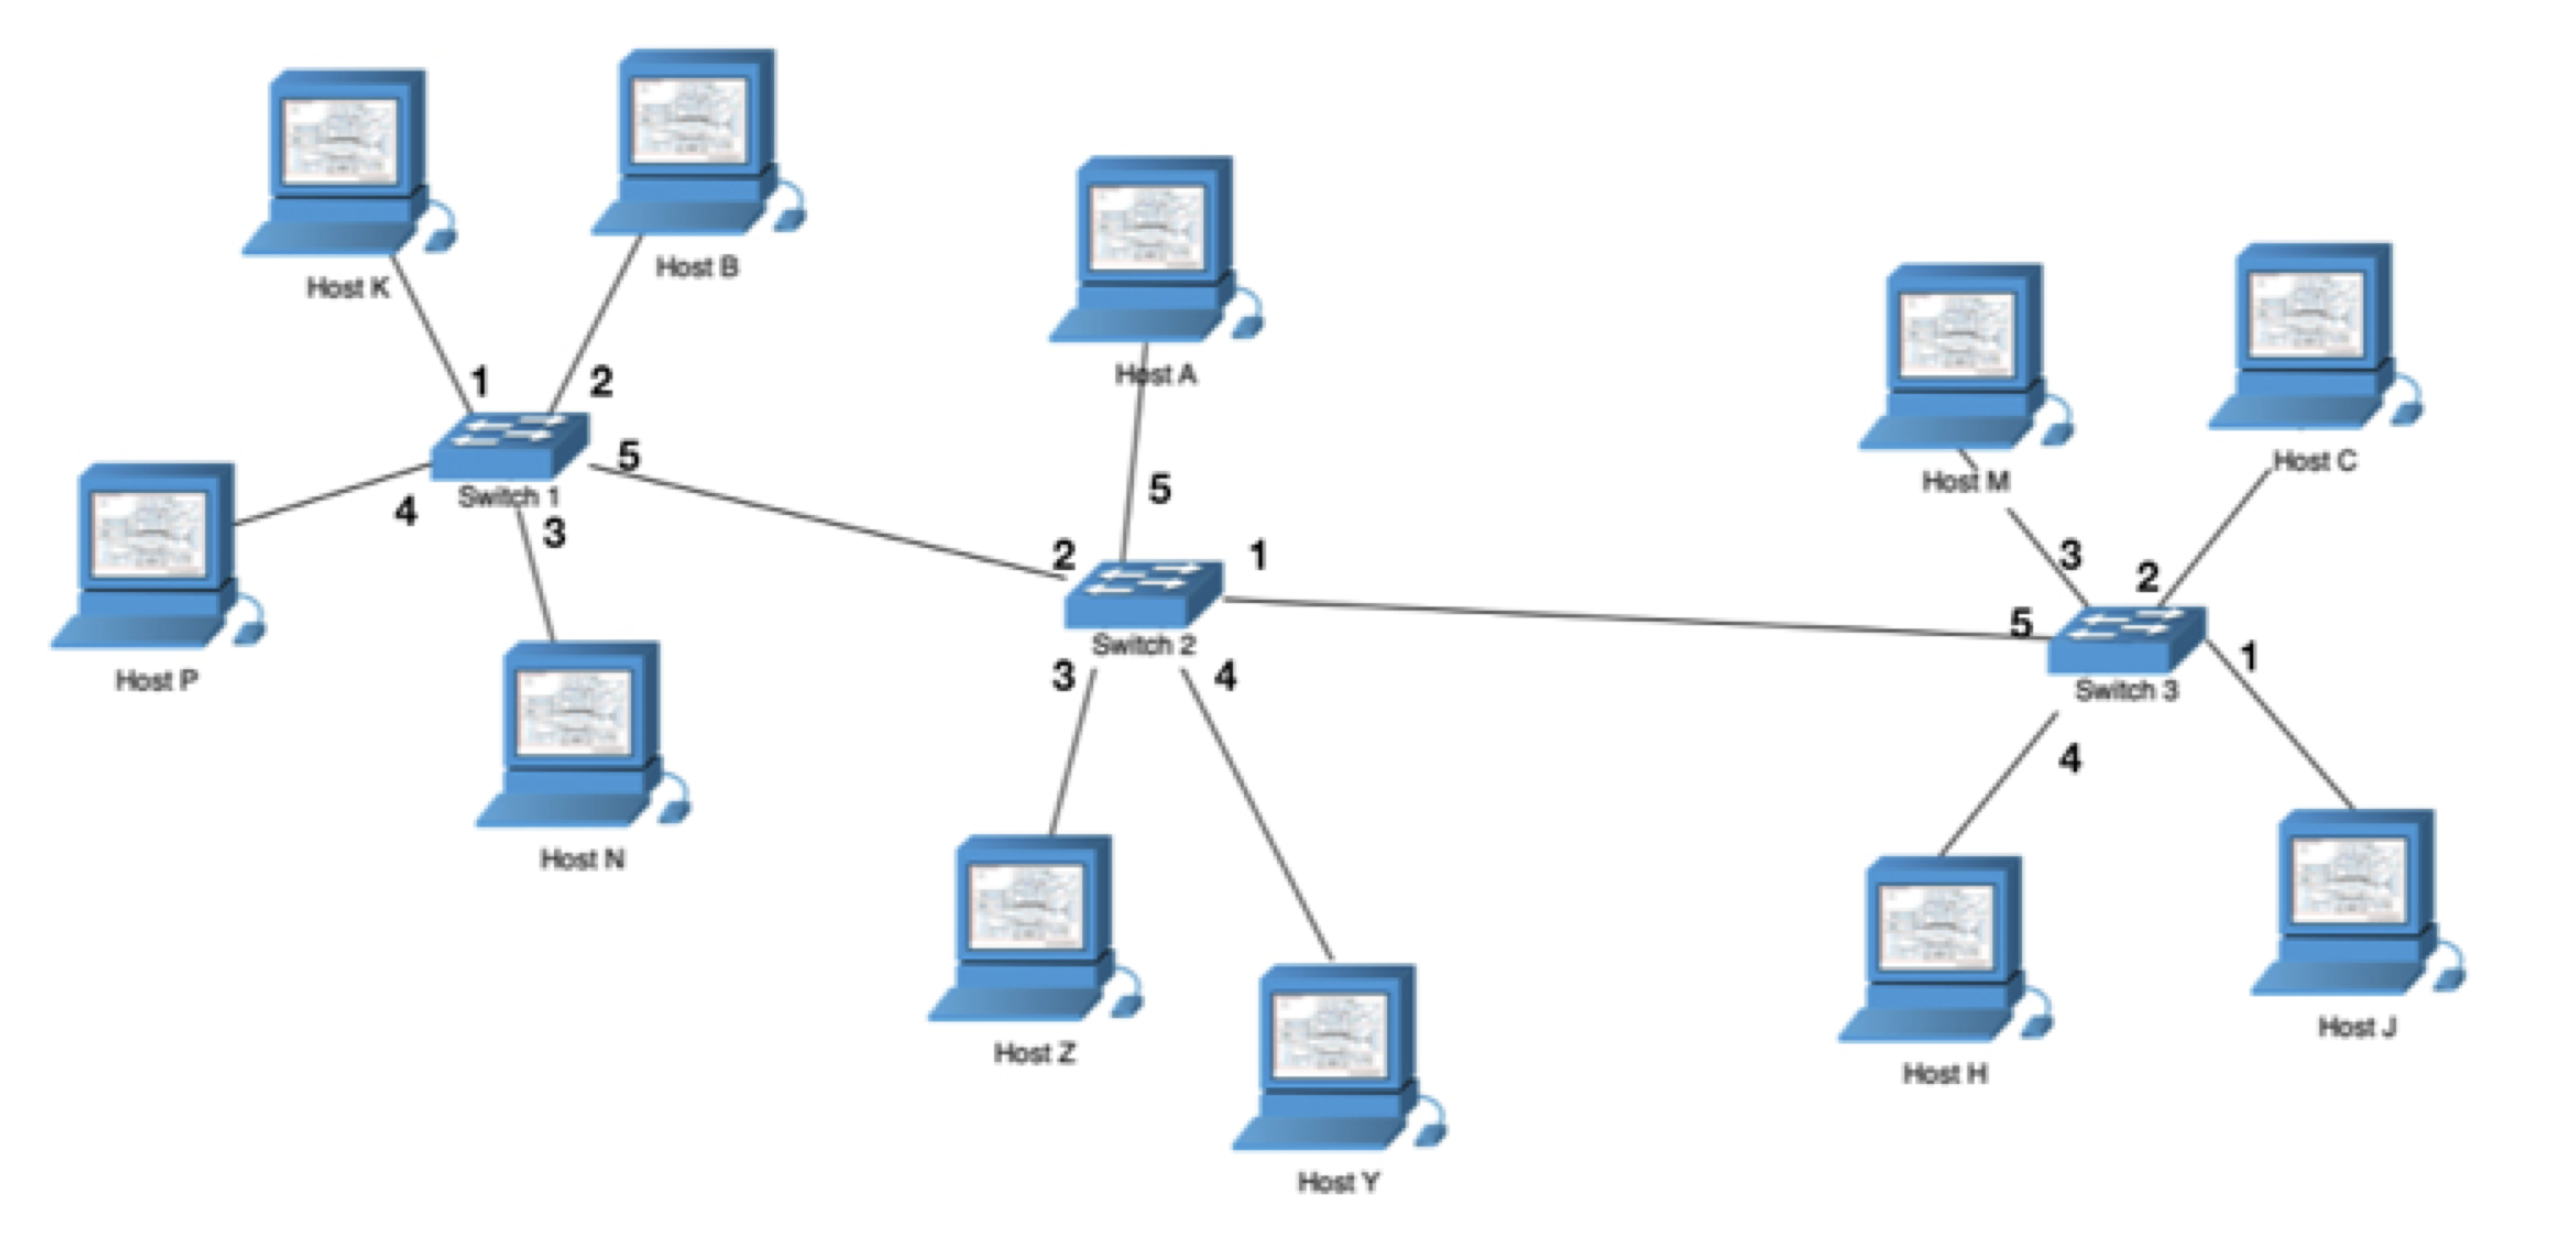
\includegraphics[width=0.9\linewidth]{fig/switches.png}\end{center}
\begin{solution}[5in]
	\begin{table}[H]
		\centering
		\caption{Solution 7}
		\label{Table 1}
		\begin{tabular}{|c|c|}
			\hline
			\multicolumn{2}{|c|}{Switch \#2}      \\ \hline
			Destination Label & Destination Port \\ \hline
			Switch 3          & 1                \\
			Switch 1          & 2                \\
			Host Z            & 3                \\
			Host Y            & 4                \\
			Host A            & 5                \\ \hline
		\end{tabular}
	\end{table}
\end{solution}


\question[12] A host launches three IP datagrams that have payloads of \SI{1280}{bytes}, \SI{1280}{bytes} and \SI{394}{bytes}. The MTU of the directly attached network is \SI{1460}{bytes}, but the destination host's network has an MTU of \SI{576}{bytes} (the ``minimum MTU'' supported by IP). Assume that these are the only two networks the datagrams must pass through. Indicate how each packet will be fragmented and specify for each fragment the size of each fragment's payload, the status of the ``more'' bit, and the value of the Offset field.
\begin{solution}[3in]
	To Switch from Host:(1460)
	\begin{enumerate}	
		\item Packet 1: 
		\begin{enumerate}
			\item Size: 1280 + 20 bytes for IP Header
			\item Fragment Offset: 0
			\item Flags: 0b000
		\end{enumerate}
		\item Packet 2: 
		\begin{enumerate}
			\item Size: 1280 + 20 bytes for IP Header
			\item Fragment Offset: 0
			\item Flags: 0b000
		\end{enumerate}
		\item Packet 3:
		\begin{enumerate}
			\item Size: 394 + 20 bytes for IP Header
			\item Fragment Offset: 0
			\item Flags: 0b000
		\end{enumerate}
	\end{enumerate}
	
	To Host from Switch: (576)
	\begin{enumerate}	
		\item Packet 1: 
		\begin{enumerate}
			\item Size: 556 + 20 bytes for IP Header
			\item Offset: 0
			\item Flags: 0b001
		\end{enumerate}
		\item Packet 2: 
		\begin{enumerate}
			\item Size: 556 + 20 bytes for IP Header
			\item Offset: 556
			\item Flags: 0b001
		\end{enumerate}
		\item Packet 3:
		\begin{enumerate}
			\item Size: 168 + 20 bytes for IP Header
			\item Offset: 1112
			\item Flags: 0b000
		\end{enumerate}
			\item Packet 4: 
		\begin{enumerate}
			\item Size: 556 + 20 bytes for IP Header
			\item Offset: 0
			\item Flags: 0b001
		\end{enumerate}
		\item Packet 5: 
		\begin{enumerate}
			\item Size: 556 + 20 bytes for IP Header
			\item Offset: 556
			\item Flags: 0b001
		\end{enumerate}
		\item Packet 6:
		\begin{enumerate}
			\item Size: 168 + 20 bytes for IP Header
			\item Offset: 1112
			\item Flags: 0b000
		\end{enumerate}
		\item Packet 7:
		\begin{enumerate}
			\item Size: 394 + 20 bytes for IP Header
			\item Offset: 0
			\item Flags: 0b000
		\end{enumerate}
	\end{enumerate}

\end{solution}
\newpage
\question[10] A device joins a network for the first time. Which sequence of messages is more logical from that device: a DHCP request followed by an ARP request, or an ARP request followed by a DHCP request? \textbf{Justify your answer.}
\begin{solution}[3in]
	First DHCP requests happen, then an ARP request happens.
	
	In the initial DHCP request (after the offer) the sender is to send back their MAC address so they the DHCP server knows what to do with it and what IP to assign (whether it can randomly assign one or the DHCP server has a static rule for said MAC).
	
	After the DHCP server receives this request it then checks to see if the given MAC is already assigned anywhere in it's ARP tables.  If not, it is free to carry on with what it was deciding to do, otherwise the DHCP server (may) ignore the request and assume it is a duplicate.  An acknowledgment is then sent back to the client, and the ARP entry is assigned.
	
	The client then will receive their new IP and submit an ARP request to verify it's newly assigned connection.  Often times after this verification completion, the client also sends another global ARP broadcast to let everyone on the network to know the host now exists. 
\end{solution}


\question[15] Shown below is a (hopefully familiar) simple network, along with the corresponding distance vectors for each node.
\begin{center}
\begin{minipage}{0.45\linewidth}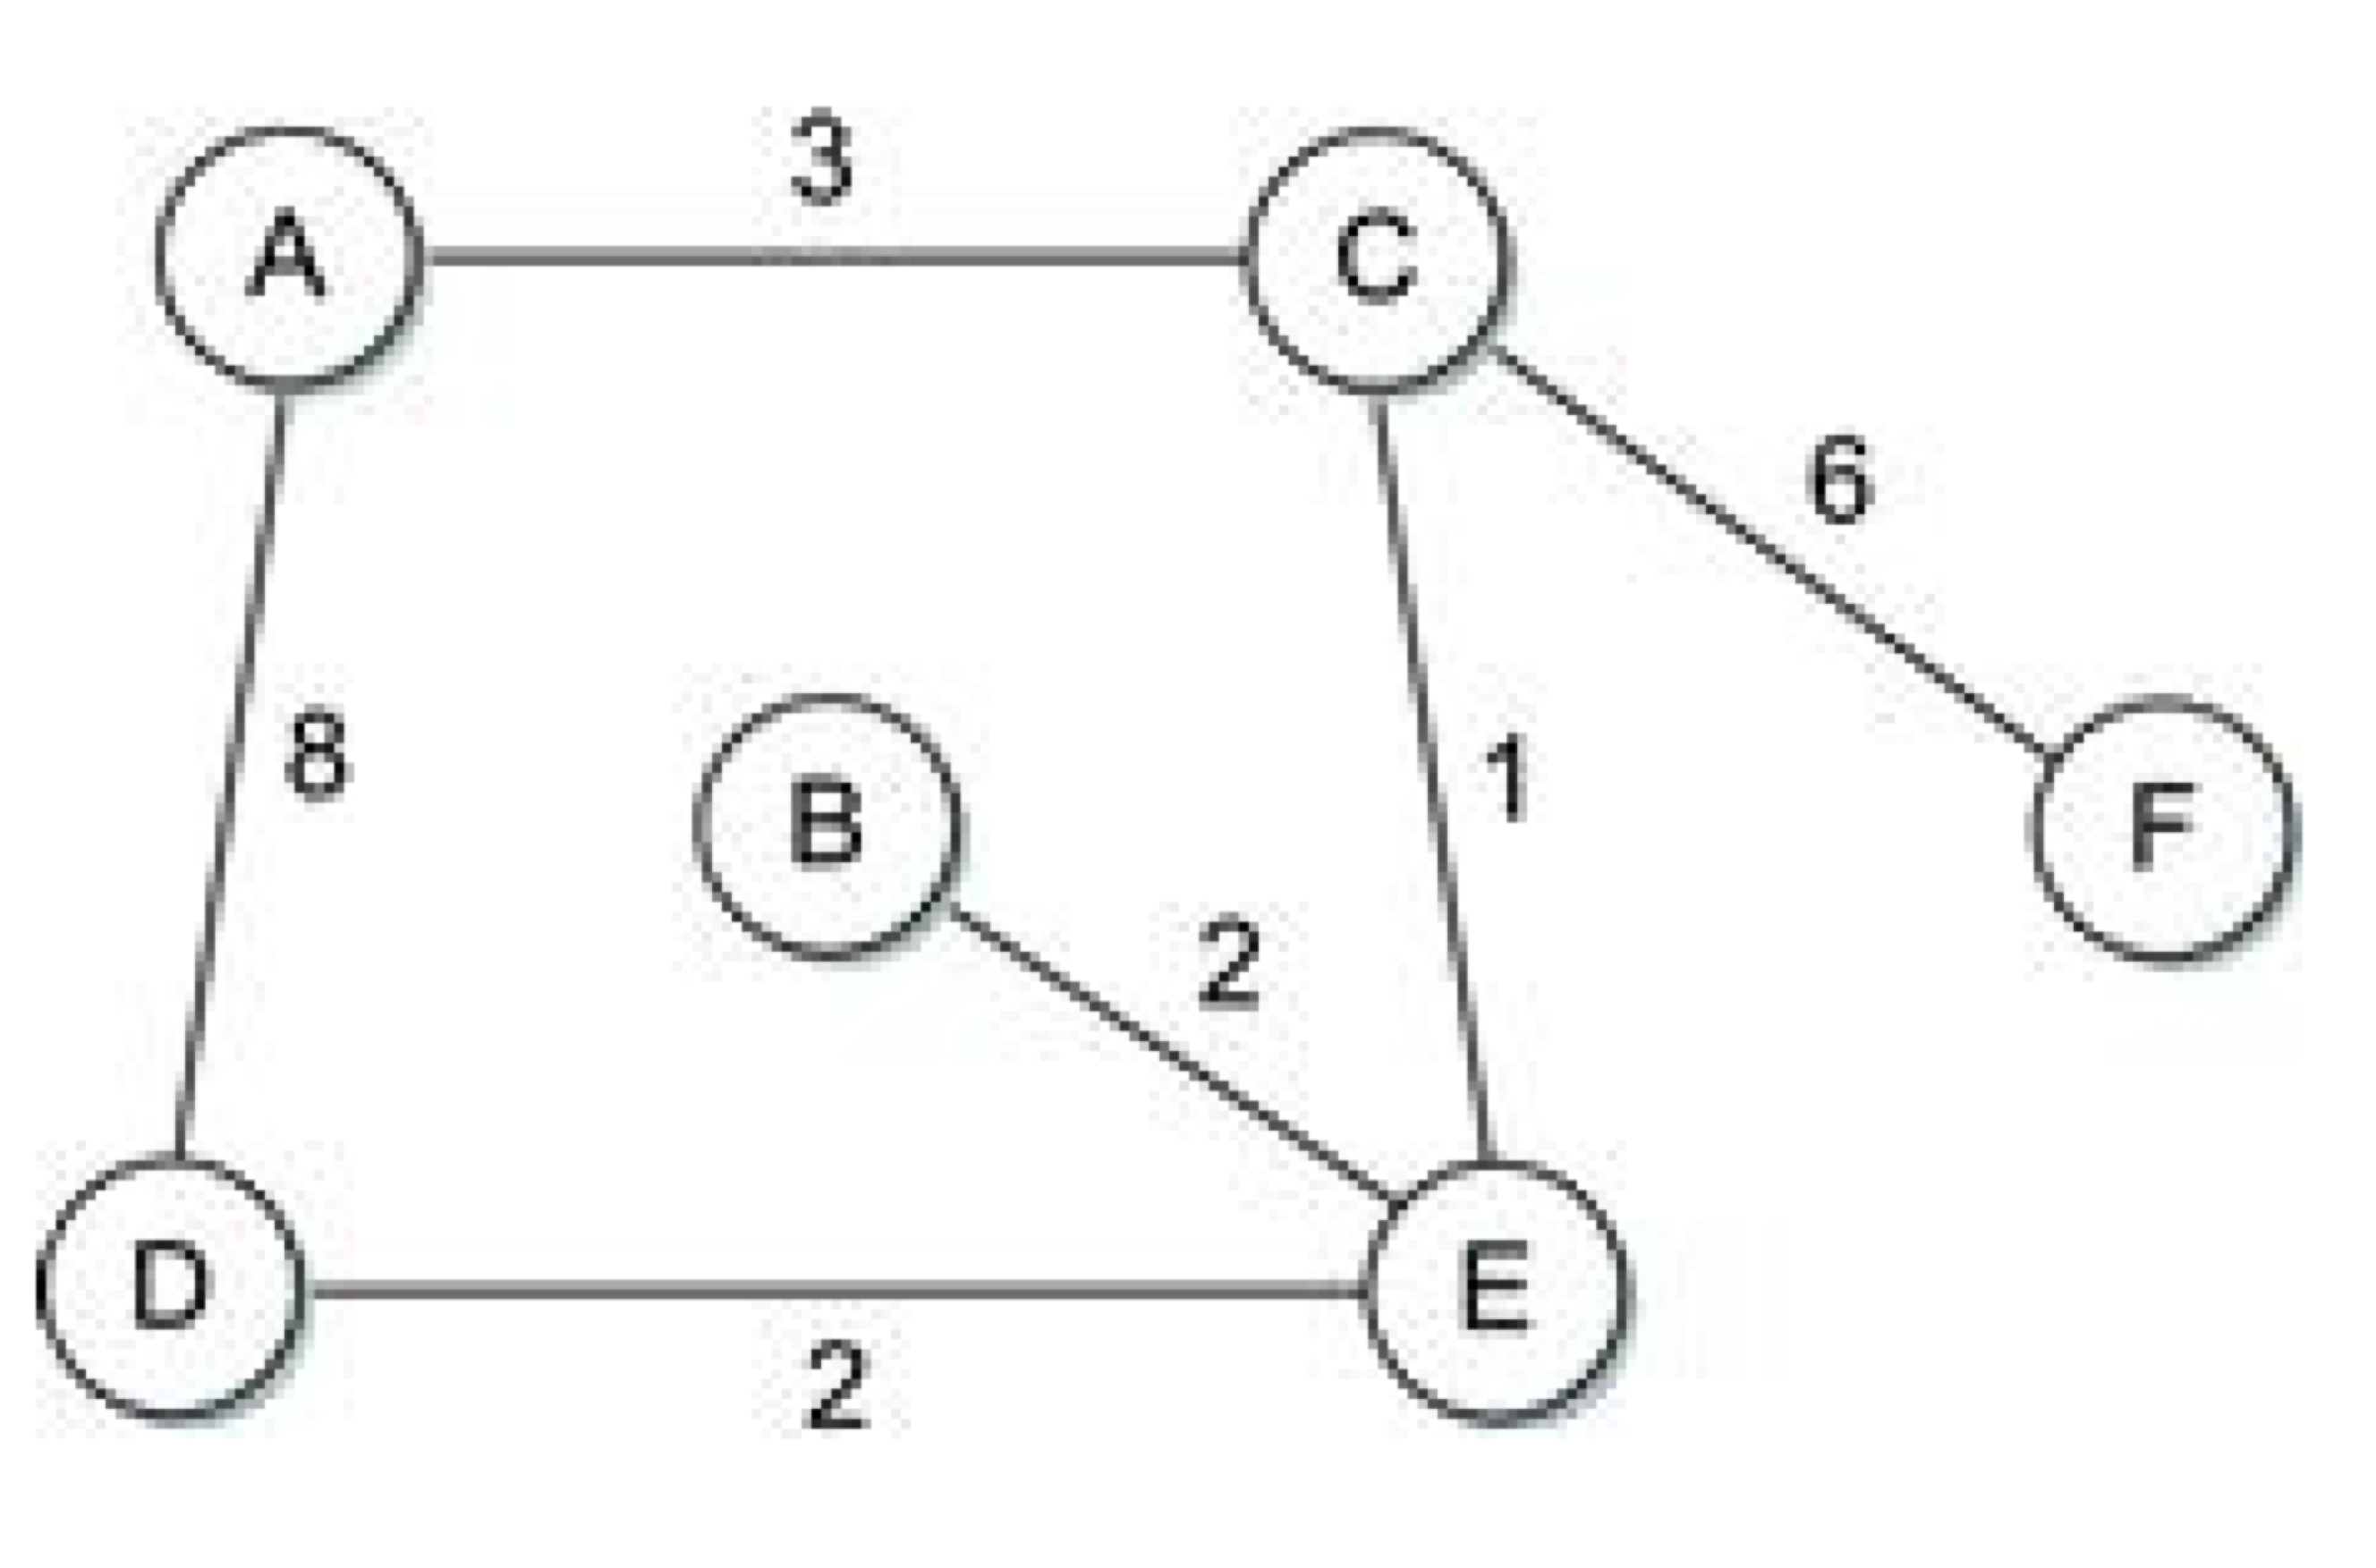
\includegraphics[width=0.9\linewidth]{fig/distance.png}\end{minipage}
\begin{minipage}{0.45\linewidth}
\begin{tabular}{c|cccccc}
\toprule
-- & A        & B        & C        & D        & E        & F        \\
\midrule
A  & --       & 6        & 3        & 6        & 4        & 9        \\
B  & 6        & --       & 3        & 4        & 2        & 9        \\
C  & 3        & 3        & --       & 3        & 1        & 6        \\
D  & 6        & 4        & 3        & --       & 2        & 9        \\
E  & 4        & 2        & 1        & 2        & --       & 7        \\
F  & 9        & 9        & 6        & 9        & 7        & --       \\
\bottomrule
\end{tabular}
\end{minipage}
\end{center}
Suppose that the link between C and E fails. Assuming no count-to-infinity problems, show the series of updates that will eventually reconnect the nodes, along with the cost of the new path between C and E. You don't need to show every table swap---just focus on the updates pertaining to the failed link.
\begin{solution}[5in]
	Updates Happening:
	\begin{enumerate}
		\item C $\rightarrow$ E changes to $\infty$
		\item E $\rightarrow$ C changes to $\infty$
		\item A $\rightarrow$ E changes to $\infty$
		\item E $\rightarrow$ A changes to $\infty$
		\item F $\rightarrow$ E changes to $\infty$
		\item E $\rightarrow$ F changes to $\infty$
		
		\item Begin restructuring as D shows a 2 unit connection to E.
		
		\item A $\rightarrow$ E changes to $10$
		\item E $\rightarrow$ A changes to $10$
		\item C $\rightarrow$ E changes to $13$
		\item E $\rightarrow$ C changes to $13$
		\item F $\rightarrow$ E changes to $19$
		\item E $\rightarrow$ F changes to $19$
	\end{enumerate}

\begin{table}[H]
	\centering
	\caption{Step 0 part A}
	\label{Solution 10}
	\begin{tabular}{|c|c|c|c|c|c|c|}
		\hline
		\multicolumn{7}{|c|}{Distance, Next Hop to Reach Node} \\ \hline
		& A   & B   & C          & D   & E          & F   \\ \hline
		A    & -   & 6   & 3          & 6   & 4          & 9   \\
		B    & 6   & -   & 3          & 4   & 2          & 9   \\
		C    & 3   & 3   & -          & 3   & 1   & 6   \\
		D    & 6   & 4   & 3          & -   & 2          & 9   \\
		E    & 4   & 2   & $\infty$   & 2   & -          & 7   \\
		F    & 9   & 9   & 6          & 9   & 7          & -  \\ \hline
	\end{tabular}
\end{table}
\begin{table}[H]
	\centering
	\caption{Step 0 part B}
	\label{Solution 10}
	\begin{tabular}{|c|c|c|c|c|c|c|}
		\hline
		\multicolumn{7}{|c|}{Distance, Next Hop to Reach Node} \\ \hline
		& A   & B   & C          & D   & E          & F   \\ \hline
		A    & -   & 6   & 3          & 6   & 4          & 9   \\
		B    & 6   & -   & 3          & 4   & 2          & 9   \\
		C    & 3   & 3   & -          & 3   & $\infty$   & 6   \\
		D    & 6   & 4   & 3          & -   & 2          & 9   \\
		E    & 4   & 2   & $\infty$   & 2   & -          & 7   \\
		F    & 9   & 9   & 6          & 9   & 7          & -  \\ \hline
	\end{tabular}
\end{table}
\begin{table}[H]
	\centering
	\caption{Question 10: Step 1  part A}
	\label{Solution 10}
	\begin{tabular}{|c|c|c|c|c|c|c|}
		\hline
		\multicolumn{7}{|c|}{Distance, Next Hop to Reach Node} \\ \hline
	   		 & A   & B   & C       & D     & E   & F   				\\ \hline
		A    & -   & 6   & 3          & 6   & 4          & 9   \\
		B    & 6   & -   & 3          & 4   & 2          & 9   \\
		C    & 3   & 3   & -          & 3   & $\infty$   & 6   \\
		D    & 6   & 4   & 3          & -   & 2          & 9   \\
		E    & $\infty$   & 2   & $\infty$   & 2   & -          & 7   \\
		F    & 9   & 9   & 6          & 9   & 7          & -  \\ \hline
	\end{tabular}
\end{table}
\begin{table}[H]
	\centering
	\caption{Question 10: Step 1  part B}
	\label{Solution 10}
	\begin{tabular}{|c|c|c|c|c|c|c|}
		\hline
		\multicolumn{7}{|c|}{Distance, Next Hop to Reach Node} \\ \hline
		& A   & B   & C       & D     & E   & F   				\\ \hline
		A    & -   & 6   & 3          & 6   & $\infty$          & 9   \\
		B    & 6   & -   & 3          & 4   & 2          & 9   \\
		C    & 3   & 3   & -          & 3   & $\infty$   & 6   \\
		D    & 6   & 4   & 3          & -   & 2          & 9   \\
		E    & $\infty$   & 2   & $\infty$   & 2   & -          & 7   \\
		F    & 9   & 9   & 6          & 9   & 7          & -  \\ \hline
	\end{tabular}
\end{table}
\begin{table}[H]
	\centering
	\caption{Question 10: Step 2  part A}
	\label{Solution 10}
	\begin{tabular}{|c|c|c|c|c|c|c|}
		\hline
		\multicolumn{7}{|c|}{Distance, Next Hop to Reach Node} \\ \hline
			 & A   & B   & C       & D     & E   & F   				\\ \hline
		A    & -   & 6   & 3          & 6   & $\infty$          & 9   \\
		B    & 6   & -   & 3          & 4   & 2          & 9   \\
		C    & 3   & 3   & -          & 3   & $\infty$   & 6   \\
		D    & 6   & 4   & 3          & -   & 2          & 9   \\
		E    & $\infty$   & 2   & $\infty$   & 2   & -          & 7   \\
		F    & 9   & 9   & 6          & 9   & $\infty$          & -  \\ \hline
	\end{tabular}
\end{table}
\begin{table}[H]
	\centering
	\caption{Question 10: Step 2  part B}
	\label{Solution 10}
	\begin{tabular}{|c|c|c|c|c|c|c|}
		\hline
		\multicolumn{7}{|c|}{Distance, Next Hop to Reach Node} \\ \hline
		     & A   & B   & C          & D     	& E   & F   				\\ \hline
		A    & -   & 6   & 3          & 6   & $\infty$          & 9   \\
		B    & 6   & -   & 3          & 4   	& 2          & 9   \\
		C    & 3   & 3   & -          & 3   	& $\infty$   & 6   \\
		D    & 6   & 4   & 3          & -   	& 2          & 9   \\
		E    & $\infty$   & 2   & $\infty$   	& 2   & -          & $\infty$   \\
		F    & 9   & 9   & 6          & 9   	& $\infty$          & -  \\ \hline
	\end{tabular}
\end{table}

\begin{table}[H]
	\centering
	\caption{Question 10: Step 3  part A \\ Begin restructuring as D shows a 2 unit connection to E.}
	\label{Solution 10}
	\begin{tabular}{|c|c|c|c|c|c|c|}
		\hline
		\multicolumn{7}{|c|}{Distance, Next Hop to Reach Node} \\ \hline
		& A   & B   & C          & D     	& E   & F   				\\ \hline
		A    & -   & 6   & 3          & 6   & 10          & 9   \\
		B    & 6   & -   & 3          & 4   	& 2          & 9   \\
		C    & 3   & 3   & -          & 3   	& $\infty$   & 6   \\
		D    & 6   & 4   & 3          & -   	& 2          & 9   \\
		E    & $\infty$   & 2   & $\infty$   	& 2   & -          & $\infty$   \\
		F    & 9   & 9   & 6          & 9   	& $\infty$          & -  \\ \hline
	\end{tabular}
\end{table}
\begin{table}[H]
	\centering
	\caption{Question 10: Step 3  part B}
	\label{Solution 10}
	\begin{tabular}{|c|c|c|c|c|c|c|}
		\hline
		\multicolumn{7}{|c|}{Distance, Next Hop to Reach Node} \\ \hline
		& A   & B   & C          & D     	& E   & F   				\\ \hline
		A    & -   & 6   & 3          & 6   & 10          & 9   \\
		B    & 6   & -   & 3          & 4   	& 2          & 9   \\
		C    & 3   & 3   & -          & 3   	& $\infty$   & 6   \\
		D    & 6   & 4   & 3          & -   	& 2          & 9   \\
		E    & 10   & 2   & $\infty$   	& 2   & -          & $\infty$   \\
		F    & 9   & 9   & 6          & 9   	& $\infty$          & -  \\ \hline
	\end{tabular}
\end{table}
\begin{table}[H]
	\centering
	\caption{Question 10: Step 4  part A}
	\label{Solution 10}
	\begin{tabular}{|c|c|c|c|c|c|c|}
		\hline
		\multicolumn{7}{|c|}{Distance, Next Hop to Reach Node} \\ \hline
		& A   & B   & C          & D     	& E   & F   				\\ \hline
		A    & -   & 6   & 3          & 6   & 10          & 9   \\
		B    & 6   & -   & 3          & 4   	& 2          & 9   \\
		C    & 3   & 3   & -          & 3   	& 13   & 6   \\
		D    & 6   & 4   & 3          & -   	& 2          & 9   \\
		E    & 10   & 2   & $\infty$   	& 2   & -          & $\infty$   \\
		F    & 9   & 9   & 6          & 9   	& $\infty$          & -  \\ \hline
	\end{tabular}
\end{table}
\begin{table}[H]
	\centering
	\caption{Question 10: Step 4  part B}
	\label{Solution 10}
	\begin{tabular}{|c|c|c|c|c|c|c|}
		\hline
		\multicolumn{7}{|c|}{Distance, Next Hop to Reach Node} \\ \hline
		& A   & B   & C          & D     	& E   & F   				\\ \hline
		A    & -   & 6   & 3          & 6   & 10          & 9   \\
		B    & 6   & -   & 3          & 4   	& 2          & 9   \\
		C    & 3   & 3   & -          & 3   	& 13   & 6   \\
		D    & 6   & 4   & 3          & -   	& 2          & 9   \\
		E    & 10   & 2   & 13   	& 2   & -          & $\infty$   \\
		F    & 9   & 9   & 6          & 9   	& $\infty$          & -  \\ \hline
	\end{tabular}
\end{table}
\begin{table}[H]
	\centering
	\caption{Question 10: Step 5  part A}
	\label{Solution 10}
	\begin{tabular}{|c|c|c|c|c|c|c|}
		\hline
		\multicolumn{7}{|c|}{Distance, Next Hop to Reach Node} \\ \hline
		& A   & B   & C          & D     	& E   & F   				\\ \hline
		A    & -   & 6   & 3          & 6   & 10          & 9   \\
		B    & 6   & -   & 3          & 4   	& 2          & 9   \\
		C    & 3   & 3   & -          & 3   	& 13   & 6   \\
		D    & 6   & 4   & 3          & -   	& 2          & 9   \\
		E    & 10   & 2   & 13   	& 2   & -          & 19   \\
		F    & 9   & 9   & 6          & 9   	& $\infty$          & -  \\ \hline
	\end{tabular}
\end{table}
\begin{table}[H]
	\centering
	\caption{Question 10: Step 5  part A}
	\label{Solution 10}
	\begin{tabular}{|c|c|c|c|c|c|c|}
		\hline
		\multicolumn{7}{|c|}{Distance, Next Hop to Reach Node} \\ \hline
		& A   & B   & C          & D     	& E   & F   				\\ \hline
		A    & -   & 6   & 3          & 6   & 10          & 9   \\
		B    & 6   & -   & 3          & 4   	& 2          & 9   \\
		C    & 3   & 3   & -          & 3   	& 13   & 6   \\
		D    & 6   & 4   & 3          & -   	& 2          & 9   \\
		E    & 10   & 2   & 13   	& 2   & -          & 19   \\
		F    & 9   & 9   & 6          & 9   	& 19          & -  \\ \hline
	\end{tabular}
\end{table}

\newpage

\vfill

\bonusquestion \textbf{(bonus)} Typically CIDR address 0.0.0.0/0 is considered invalid. Assume we want to instead implement our software-defined network to support 0.0.0.0/0: should it match every IP address, or no IP address? While there is no correct decision, be sure to \textbf{justify your answer} with a short (sentence of two) reasoning using appropriate terminology.
\end{solution}


\begin{solution}[1in]
	I would say that 0.0.0.0/0 should be valid for all IPV4 addresses.  My reasoning for this is essentially just due to that is how the math itself works out. 
	\begin{center}
		$\textrm{Addr: }$ 00000000.00000000.00000000.00000000
		
		$\textrm{Mask: }$ 00000000.00000000.00000000.00000000
		
		$\textrm{Wild: }$ 11111111.11111111.11111111.11111111
		
		$\textrm{Minimum Host: }$ 0.0.0.1
		
		$\textrm{Maximum Host: }$ 255.255.255.254
		
		$\textrm{Broadcast: }$ 255.255.255.255
	\end{center}
	As another reason that it would make sense, is that it would seem odd to not have a CIDR notation that could cover all potential IP addresses as it would breakup the flow of many charts and data address fields as an "allow all" option would have to be something not in CIDR notation adding extra annoyances.
\end{solution}
\end{questions}

\newpage
\begin{center}\hrulefill\\\textcolor{gray}{Scratch Work}\end{center}
\vfill
\begin{center}\gradetable[v][questions]\end{center}

\end{document}
